\newcommand{\texCommand}[1]{\texttt{\textbackslash{#1}}}%

\newcommand{\exemplo}[1]{%
\vspace{\baselineskip}%
\noindent\fbox{\begin{minipage}{\textwidth}#1\end{minipage}}%
\\\vspace{\baselineskip}}%

\newcommand{\exemploVerbatim}[1]{%
\vspace{\baselineskip}%
\noindent\fbox{\begin{minipage}{\textwidth}%
#1\end{minipage}}%
\\\vspace{\baselineskip}}%

Este capítulo descreve toda a fundamentação teórica por trás das tecnologias utilizadas na implementação do estudo de caso. Inicialmente, explico os conceitos gerais relacionados a teoria de grafos, em seguida, aponto as principais características e utilidades dos SGBDs NoSQL. Posteriormente, aponto as características e particularidades de um SGBD orientado a grafos, junto com uma explicação acerca do SGBD escolhido para o trabalho que é o OrientDB. Por fim, explico um pouco sobre a tecnologia REST utilizada para a comunicação entre o sistema desenvolvido e o OrientDB.

%%%%%%%%%%%%%%%%%%%%%%%%%%%%%%%%%%%%%%%%%%%%%%%%%%%%%%%%%%%%%%%%%%%%%%%%%%%%%%%%
%%%%%%%%%%%%%%%%%%%%%%%%%%%%%%%%%%%%%%%%%%%%%%%%%%%%%%%%%%%%%%%%%%%%%%%%%%%%%%%%
%%%%%%%%%%%%%%%%%%%%%%%%%%%%%%%%%%%%%%%%%%%%%%%%%%%%%%%%%%%%%%%%%%%%%%%%%%%%%%%%
\section{Teoria de Grafos} \label{graph_theory}
	Essa seção, aborda a teoria por trás da estrutura de um grafo, necessária para a compreensão do funcionamento de um SGBD orientado a grafos. Qualquer SGBD orientado a grafos utiliza algum dos conceitos aqui descritos para a construção do banco de dados.

\subsection{Definição de um grafo}
	A definição formal de um grafo pode ser feita da seguinte forma: Um grafo \(G\) é uma tripla ordenada \((V(G), E(G), \psi g)\), que consiste de um conjunto não vazio \(V(G)\) de vértices, um conjunto \(E(G)\), disjunto do conjunto \(V(G)\), de arestas, e uma função de incidência \(\psi g\) que associa cada aresta de \(G\) um par não ordenado (não necessáriamente distinto) de vértices de \(G\). Dessa forma, se \(e\) é uma aresta e \(u\) e \(v\) são vértices, de tal modo que \(\psi g(e) = uv\), então, diz-se que \(e\) faz a união de \(u\) e \(v\); Os vértices \(u\) e \(v\) são chamados de extremidades de \(e\) \cite{bondy1976graph}.
	
	A figura \ref{graph_definition} esclarece a definição fornecida no parágrafo acima:
	
\begin{figure}[H]
	\centering
    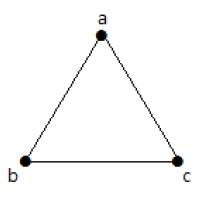
\includegraphics[width=0.8\textwidth]{simple_graph}
    \caption{Exemplo de uma estrutura de grafo}
    \label{graph_definition}
\end{figure}

	Portanto, o conjunto \(V(G)\) de vértices é não vazio e composto por três vértices, \(V(G)=\{a,b,c\}\). Já o conjunto \(E(G)\) de arestas é composto por três arestas, \(E(G)=\{e1,e2,e3\}\). De forma que a função de incidência \(\psi g\) é definida da seguinte maneira: \(\psi g(e1)= ab\), \(\psi g(e2)= ac\) e \(\psi g(e3)= bc\). Portanto, a definição formal do grafo acima é \((\{a,b,c\}, \{e1,e2,e3\}, \psi g(e1)= ab\), \(\psi g(e2)= ac\) \(\psi g(e3)= bc)\).
	
\subsection{Propriedades de um grafo}
	Um grafo possui essa nomenclatura pois pode ser representado graficamente, e a partir dessa representação é possível observar algumas propriedades importantes. Como mostra a figura \ref{graph_definition}, cada vértice é representado por um ponto, e cada aresta é representada por uma linha, juntando dois pontos \cite{bondy1976graph}. Todo grafo possui as propriedades de ordem e tamanho. A ordem de um grafo se refere ao número de vértices, ou seja, a quantidade de elementos no conjunto \(V(G)\), enquanto o tamanho de um grafo é referente ao número de arestas, ou seja, a quantidade de elementos no conjunto \(E(G)\).
	
	Boa parte da teoria de grafos é baseada em uma categoria específica que é a categoria de grafos simples. Antes de definir um grafo como simples, é necessário definir o que é um laço em um grafo. Intuitivamente, um laço é quando a aresta sai de um vértice e termina no próprio vértice. A figura \ref{graph_loop} exemplifica um laço em grafo: 

\begin{figure}[H]
	\centering
    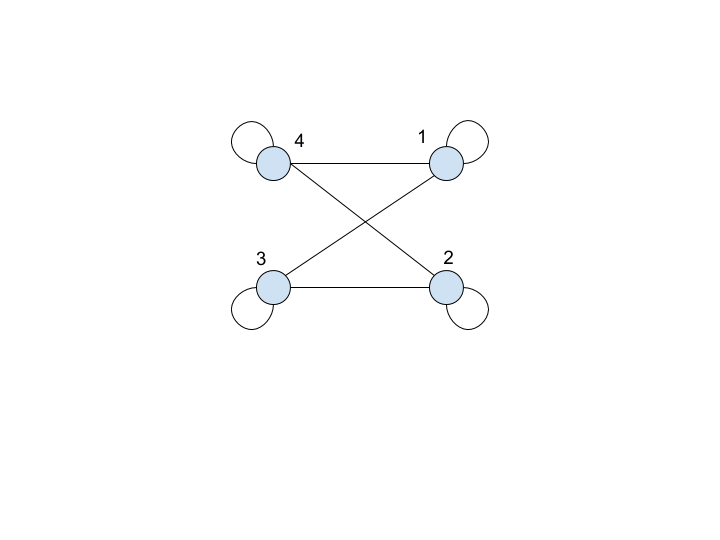
\includegraphics[width=0.4\textwidth]{graph_loop}
    \caption{Exemplo de uma estrutura de grafo com presença de laço}
    \label{graph_loop}
\end{figure}

	Dessa forma, um grafo é definido como simples se não possui laços nem duas ou mais arestas ligando dois vértices \cite{bondy1976graph}. Portanto, o grafo \ref{graph_loop} não é um grafo simples, enquanto o grafo \ref{graph_definition} é um grafo simples. Uma propriedade básica de um vértice é o seu grau. O grau de um vértice é a quantidade de aretas incidentes nele. Por exemplo, no grafo \ref{graph_definition} o vértice \(a\) possui grau 2.
	
	O grafo \ref{graph_definition}, mostra uma categoria de grafos que não faz distinção entre a orientação das arestas. Um grafo que evidencia a orientação das arestas é dito grafo orientado, como mostra a Figura \ref{graph_direction}:
	
\begin{figure}[H]
	\centering
    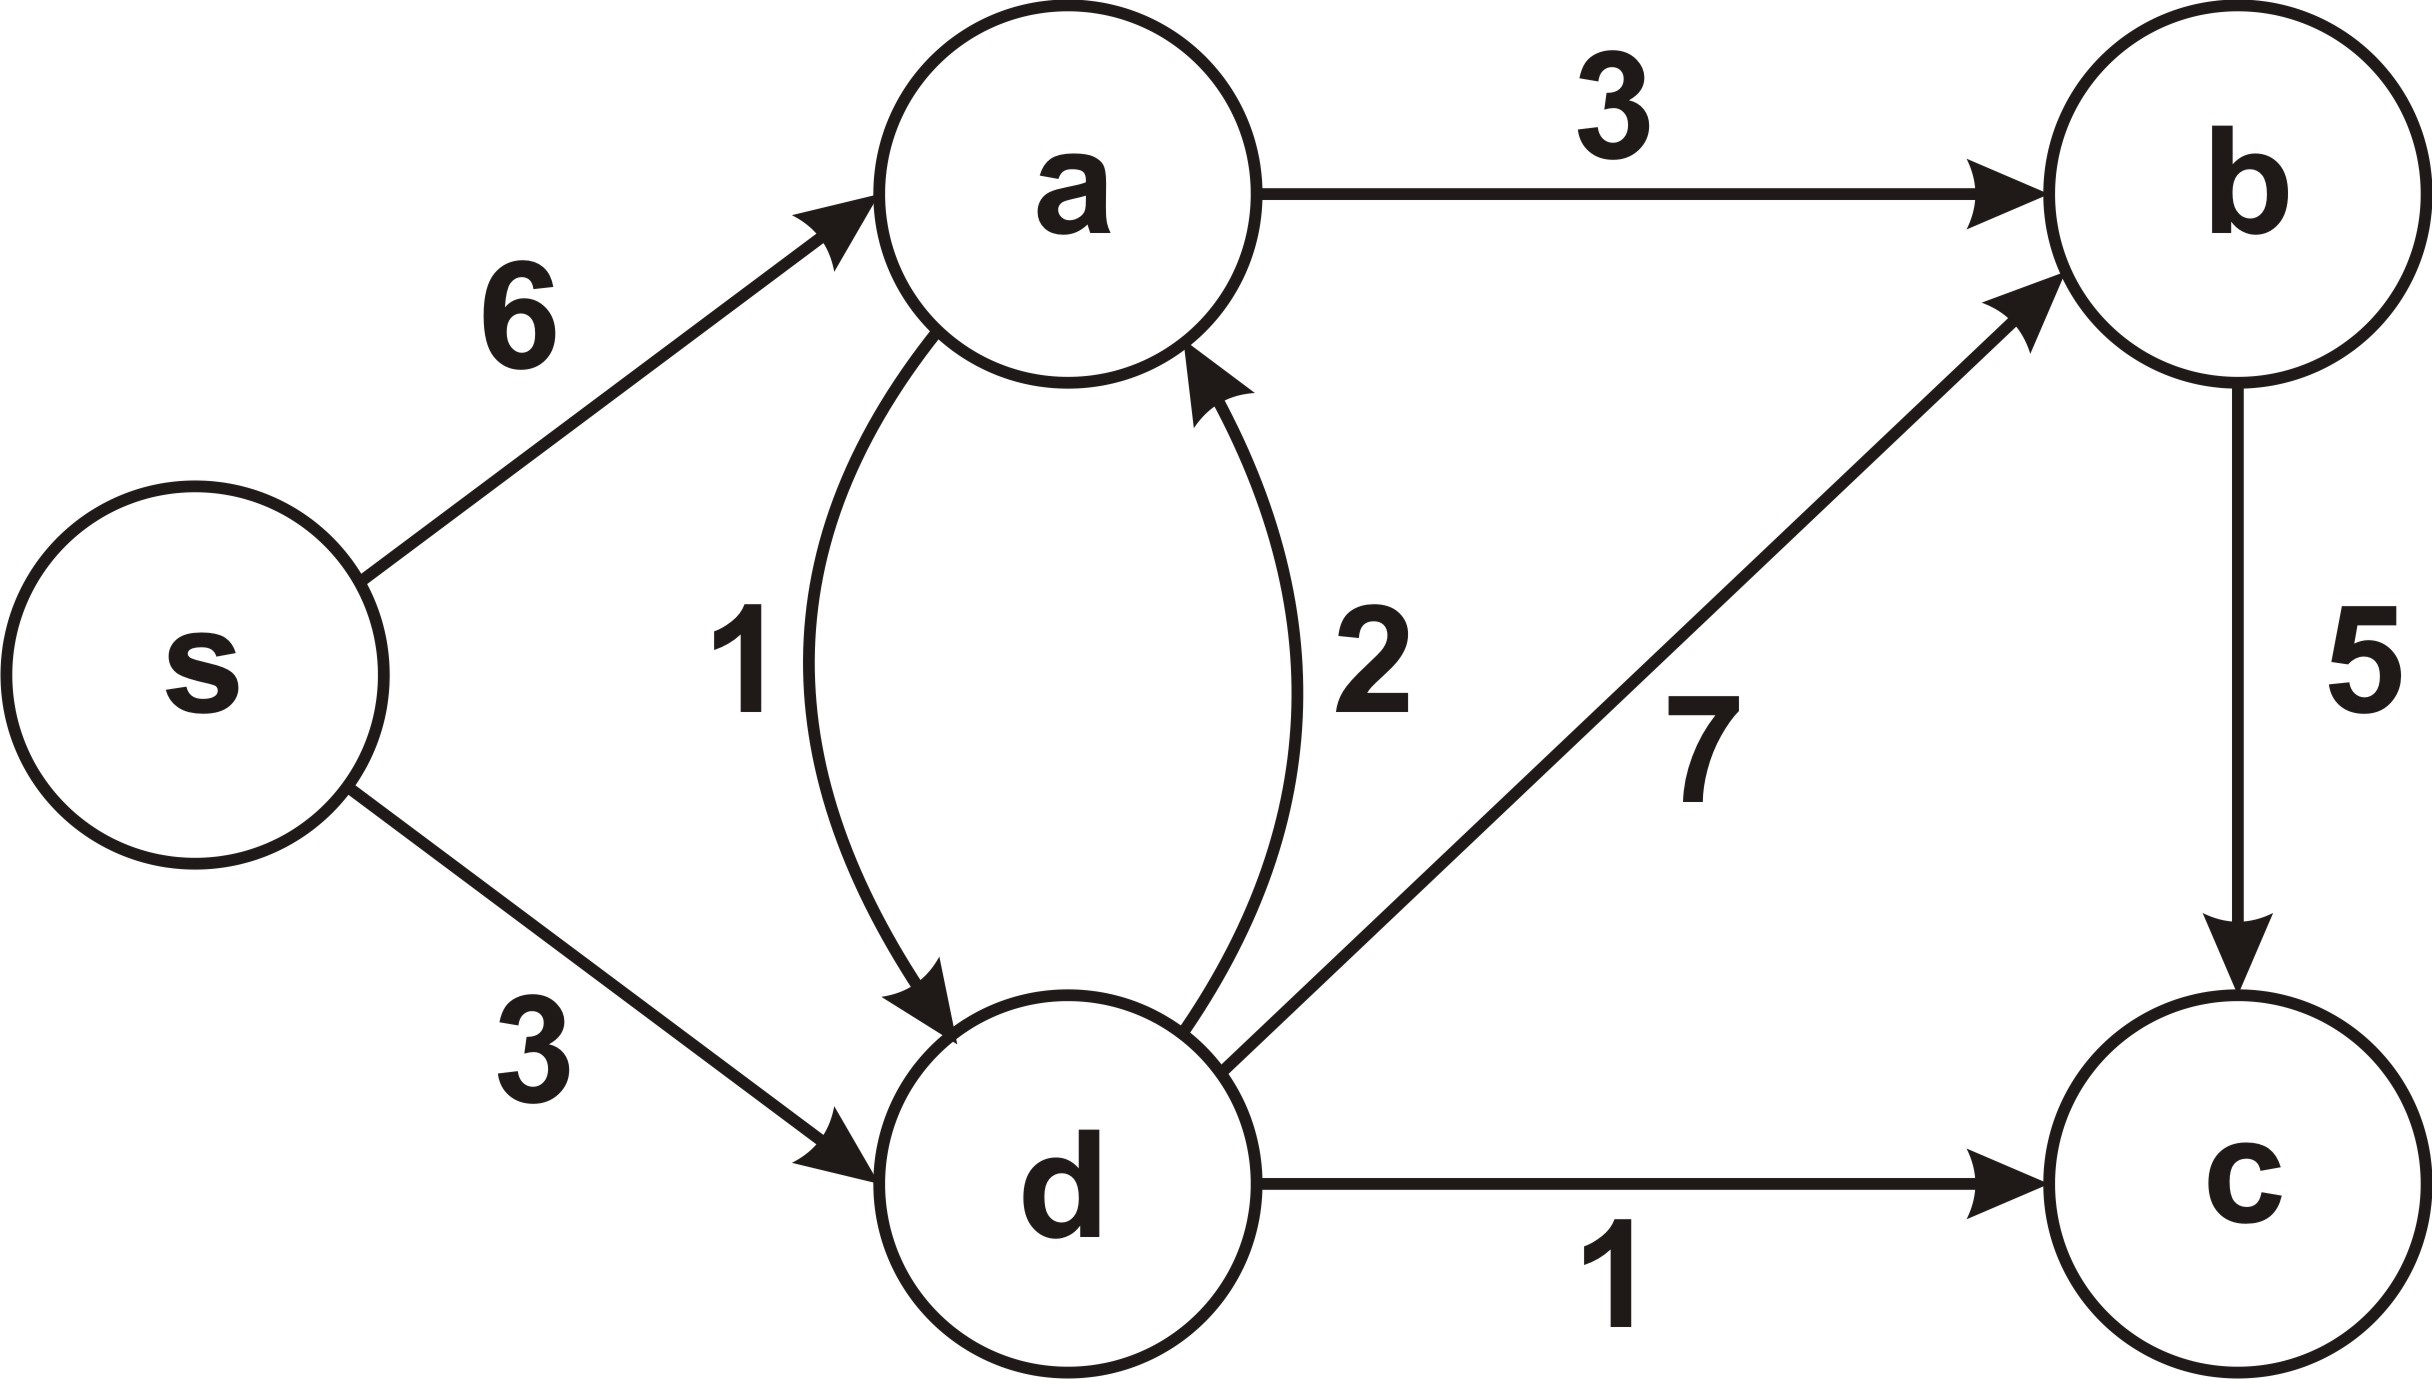
\includegraphics[width=0.4\textwidth]{direction}
    \caption{Exemplo de uma estrutura de grafo direcionado}
    \label{graph_direction}
\end{figure}

	O OrientDB utiliza grafos orientados para representar os dados. Alguns relacionamentos exigem que a direção da aresta aponte para os dois lados, o OrientDB representa essa característica com somente uma aresta e uma seta em cada extremidade, mas é importante ressaltar que o correto é representar com duas arestas, uma em cada sentido, como mostra a figura \ref{graph_direction} nas arestas 1 e 2.
	
	Dentro do universo de teoria de grafos, existem ainda diversas outras propriedades tais como: Isomorfismo entre grafos, subgrafos, caminho, caminho fechado e etc. Essas propriedades fornecem a base para a compreensão e resolução de problemas importantes para a computação, como o problema de menor caminho, que busca encontrar o menor caminho entre dois vértices em um grafo com pesos. O SGBD utilizado nesse trabalho o OrientDB, fornece uma solução para o problema de menor caminho, e conhecer a teoria por trás do problema faz com que o usuário possa usar da melhor maneira essa solução \cite{orientShortestPath}.
	
\subsection{Grafos em SGBD NoSQL}
	A teoria de grafos é um campo vasto na ciência da computação, e ao utilizar essa estrutura para armazenar dados, cada SGBD escolhe a estrutura mais adequada para atingir os objetivos definidos. O trabalho realizado por Angles \cite{angles2012comparison}, e citado por Gustavo \cite{mdgnosql} mostra que os SGBD NoSQL orientado a grafos podem ser classificados de acordo com as características de seus vértices, arestas e do próprio grafo: 
	
	Classificação pelas características do grafo:
\begin{itemize}
		\item Grafo simples: Nesse formato, cada vértice e aresta possui somente um rótulo que os identifica.
		\item Hipergrafo: Nesse formato, é permitido que suas arestas apontem para mais de dois vértices.
		\item Grafo com atributos: Nesse formato, é permitido que os vértices possuam atributos, tais atributos representam a informação de um certo dado armazenado.
		\item Grafo aninhado: Nesse formato, o grafo permite que um vértice seja outro grafo.
\end{itemize}

	Classificação pelas características do vértice:
\begin{itemize}
		\item Vértice rotulado: Nesse formato, cada vértice possui somente um rótulo que o identifica.
		\item Vértice com atributo: Nesse formato, o vértice possui atributos como um par chave-valor, por exemplo.
\end{itemize}

	Classificação pelas características da aresta:
\begin{itemize}
		\item Aresta rotulada(direcionada ou não): Nesse formato, cada aresta possui somente um rótulo que o identifica e expressa uma informação, como o relacionamento.
		\item Aresta com atributo(direcionada ou não): Nesse formato, cada aresta possui atributos sobre o vínculo.
\end{itemize}

	De acordo com essas classificações, tanto o Neo4j quanto o OrientDB utilizam a estrutura de vértices e arestas com atributos para organizar o armazenamento de dados. Conforme Gustavo \cite{mdgnosql} aponta em sua tese de mestrado, essa estrutura facilita o acesso as informações do vértice, uma vez que os atributos podem ser armazenados junto com os próprios vértices e arestas. Entranto, é importante tratar com cuidado essa propriedade, pois ao adicionar uma informação como atributo, em vez de adicionar como vértice, podem surgir problemas de identificação de relacionamentos compartilhados, pois o atributo vai estar repetido em outra instância, e para identificar esse relacionamento se faz necessário uma consulta parecida com a de um SGBD relacional \cite{mdgnosql}.
	
	Uma comparação entre o Neo4j e OrientDB é feita em mais detalhes na seção \ref{comparison_graph_nosql}, levando em conta outros aspectos além do formato de grafo utilizado para o armazenamento dos dados.
	
%%%%%%%%%%%%%%%%%%%%%%%%%%%%%%%%%%%%%%%%%%%%%%%%%%%%%%%%%%%%%%%%%%%%%%%%%%%%%%%%
%%%%%%%%%%%%%%%%%%%%%%%%%%%%%%%%%%%%%%%%%%%%%%%%%%%%%%%%%%%%%%%%%%%%%%%%%%%%%%%%
%%%%%%%%%%%%%%%%%%%%%%%%%%%%%%%%%%%%%%%%%%%%%%%%%%%%%%%%%%%%%%%%%%%%%%%%%%%%%%%%
\section{SGBD NoSQL}
	Essa seção aborda a categoria de bancos de dados não relacionais. Inicialmente, realizo uma introdução sobre o assunto, para em seguida explicitar as principais características e categorias dentro desse grupo de bancos de dados.
	
\subsection{Introdução}
	O termo NoSQL foi utilizado na literatura pela primeira vez por Carlo Strozzi em 1998 como o nome de um banco de dados que ele estava desenvolvendo na época \cite{FirstNoSQL}. Curiosamente, é um banco relacional que não possuia interface SQL, portanto, NoSQL. Entre o período dos anos de 2000 e 2005 o universo dos SGBD NoSQL começou a aumentar bastante, o SGBD baseado em grafo Neo4j começou a ser desenvolvido no ano de 2000, o SGBD da Google BigTable\cite{Chang:2008:BDS:1365815.1365816} começa em 2004 e em seguida o CouchDB se inicia por volta de 2005. Porém, todas essas tecnologias não eram na época categorizadas como NoSQL, somente em 2009 o termo foi reintroduzido por Johan Oskarsson ao organizar um evento para discutir sobre banco de dados não relacionais, distribuídos e de código aberto, e a partir desse momento o termo passa a ser usado para categorizar os bancos de dados não relacionais.
	
	O termo NoSQL gera muita confusão pois leva a entender que os bancos de dados nessa categoria não utilizam a linguagem SQL. Porém, o termo costuma ser utilizado como \textit{Not only SQL}, e demonstra que tais sistemas podem suportar também linguagens de consultas baseadas em SQL. O aspecto mais importante por trás dos SGBD NoSQL é o motivo de seus surgimentos. No início dos anos 2000, a forma como os usuários começaram a interagir na internet começou a evoluir e consequentemente os sistemas e aplicações passaram a gerar e consumir cada vez mais dados e informações. Esse crescimento na geração e consumo de dados foi enorme, e por isso os especialistas necessitavam de tecnologias que atendessem melhor suas necessidades, desse cenário começaram a nascer os primeiros SGBD NoSQL como o BigTable da google e o Dynamo da Amazon\cite{DeCandia:2007:DAH:1323293.1294281}.
	
\subsection{Características de um SGBD NoSQL}
	Como foi mencionado acima, por volta dos anos 2000 começou a nascer a necessidade de novas tecnologias na área de banco de dados. Os sistemas precisavam de boa escalabilidade horizontal para operações de forma distribuída, entre outras coisas. Vários aspectos relacionados a categoria dos SGBD NoSQL são ainda abertos e não possuem um consenso. O trabalho feito por Rick Cattell\cite{Cattell:2011:SSN:1978915.1978919} aglomerou algumas características que geralmente se encontram nesse tipo de banco de dados: 
	\begin{itemize}
		\item Habilidade de escalar horizontalmente operações simples através de vários servidores
		\item Habilidade de replicar e distribuir os dados através de vários servidores
		\item Um modelo de concorrência mais flexível que as transações ACID presentes em sistemas relacionais.
		\item Uso eficiente de índices distribuidos e da memória RAM para armazenar os dados
		\item Habilidade de adicionar dinamicamente novos atributos a um registro
	\end{itemize}
	
	Porém, é importante ressaltar que nem todas essas características precisam ser atendidas para fazer parte dessa categoria. Sendo que também existem outras características importantes observadas em alguns sistemas como por exemplo, disponibilidade e consistência dos dados, níveis de flexibilidade para o esquema do banco de dados e etc.

\subsection{Gerenciamento de Transações} \label{manage_transaction}
	Uma propriedade importante em qualquer SBGD é o controle de concorrência. Normalmente, vários usuários solicitam operações ao SGBD simultâneamente, sendo que esse sistema gerenciador de banco de dados precisa garantir aos usuários a integridades dos dados transacionados. A maioria dos bancos de dados relacionais utilizam transações ACID\cite{SistemaDeBd} para controlar essa concorrência, que impõe ao SGBD as seguintes propriedades:
	\begin{itemize}
		\item Atomicidade: Essa propriedade impôe que durante uma transação, todas as alterações feitas no banco de dados sejam efetivadas. Caso ocorra algum erro durante a transação o SGBD realiza um \textit{rollback} para o estado consistente anterior a transação.
		\item Consistência: Essa propriedade impôe que ao término de uma transação o banco de dados está de forma consistente. Ou seja, a cada transação os dados devem estar consistentes e a garantia de que as restrições impostas aos dados não sejam violadas.
		\item Isolamento: A propriedade de isolamento de uma transação, busca impor ao SGBD que cada transação seja independente das demais. Ou seja, garante que cada transação seja vista como uma unidade e impede que outras transações acessem dados que possam levar o bancos de dados a um estado inconsistente. 
		\item Durabilidade: A durabilidade garante que as informações salvas após cada transação permaneçam no banco de dados. Os dados não podem desaparecer em nenhum momento e devem permanecer persistidos independente de qualquer falha.
	\end{itemize}
	
	Esse formato é utilizado por bancos de dados relacionais, e atende bem uma boa parte de sistemas e aplicações nos dias de hoje, como é o caso de sistemas bancários por exemplo, que necessitam dessas propriedades para garantir a integridades das informações de seus clientes.
	
	O mais importante a se perceber aqui é que nem toda aplicação precisa necessariamente desse controle de concorrência elaborado. No caso de bancos é de suma importância esse tipo de controle, agora em uma aplicação de alta disponibilidade uma propriedade como a consistência pode ser um pouco mais fraca. Portanto, para atender a essas novas demandas, nasceu o modelo de transações BASE\cite{Pritchett:2008:BAA:1394127.1394128} que busca fornecer maior flexibilidade para esses novos sistemas. O BASE tem como característica em vez de exigir consistência após cada transação, é suficiente para o banco de dados estar eventualmente consistente. Existe um teorema famoso feito por Eric Brewer conhecido como Teorema CAP\cite{Brewer:2010:CFT:1835698.1835701}, que demonstra o trade-off entre consistência, disponibilidade e tolerância a particionamento. Eric diz que se for necessário essas três características, é necessário escolher somente duas delas. Portanto no modelo BASE é possíve escolher tolerância a particionamento e disponibilidade e abrir mão de uma alta consistência dos dados. O acrônimo BASE vem das três seguintes características:
	\begin{itemize}
		\item \textit{Basic Availability}: Essa propriedade no fundo quer dizer que o banco de dados aparenta funcionar a maior parte do tempo.
		\item \textit{Soft state}: Essa propriedade quer dizer que as bases não precisam estar sempre consistentes, nem as réplicas precisam estar consistentes o tempo inteiro. Ou seja, o estado do sistema é volátil.
		\item \textit{Eventual consistency}: Essa propriedade diz que as bases de dados vão ficar eventualmente consistentes no futuro. 
	\end{itemize}
	
\subsection{Categorias de NoSQL}
	Dentro do universo dos SGBD NoSQL, existem cinco grandes categorias que separam cada SGBD em relação a estratégia de armazenamento\cite{nayak2013type}. Tais categorias são:
	
\subsubsection{SGBD NoSQL por chave/valor}
	Os SGBD dessa categoria são de certa forma bem simples, mas bastante eficientes. O dado armazenado é composto por uma \textit{string} que representa a chave, e o dado de fato a ser referenciado pela chave que é o valor, portanto, se cria um par chave/valor \cite{nayak2013type}\cite{kauremerging}.
	
	Os SGBD NoSQL por chave e valor, costuma valorizar uma maior escalabilidade em troca de consistência, tal característica é mecionada na seção \ref{manage_transaction}. O seu uso é bastante eficiente para situações como guardar seções de usuário, ou gerenciar um carrinho de compras online \cite{nayak2013type}. Um exemplo de SGBD dessa categoria é o DynamoDB \cite{DeCandia:2007:DAH:1323293.1294281}. A figura abaixo mostra o formato de um dado nesse SGBD em contraste com o formato de SGBD relacional e de SGBD orientado a documentos.
	
\begin{figure}[h]
	\centering
    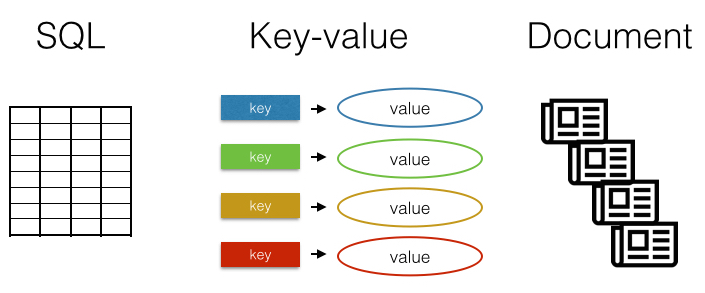
\includegraphics[width=0.8\textwidth]{key-value}
    \caption{Exemplos de estrura relacional, chave/valor e orientada a documentos}
    \label{fig:key-value}
\end{figure}
	
\subsubsection{SGBD NoSQL orientado por colunas}
	Os SGBD dessa categoria, podem ser confundidos de certa forma com um SGBD relacional por serem orientado a colunas. Mas na verdade um SGBD NoSQL orientado por colunas tem um formato híbrido entre linha e coluna. Apesar de compartilharem do conceito de armazenamento por colunas, esses SGBD não armazenam os dados em tabelas, e sim em grandes arquitetura distribuídas. Nessa categoria, cada chave é associada com uma ou mais colunas, chamada de atributos. Esse armazenamento é feito de forma que o dado seja agregado mais rapidamente e com menos processamento de entrada e saída \cite{nayak2013type}.
	
	Ou seja, esses banco de dados contém uma coluna extensível de dados fortemente relacionados, em vez de conjuntos de informação em uma estrutura rígida de tabela com linha e colunas como no modelo relacional\cite{kauremerging}. Esse tipo de NoSQL é bastante útil para operações de mineração de dados e aplicações de análise \cite{nayak2013type}. Dois grandes representantes dessa categoria são o BigTable da google \cite{Chang:2008:BDS:1365815.1365816} e o Cassandra. A figura abaixo exemplifica a diferença da estrutura orientada a colunas e orientada a documentos:
	
\begin{figure}[h]
	\centering
    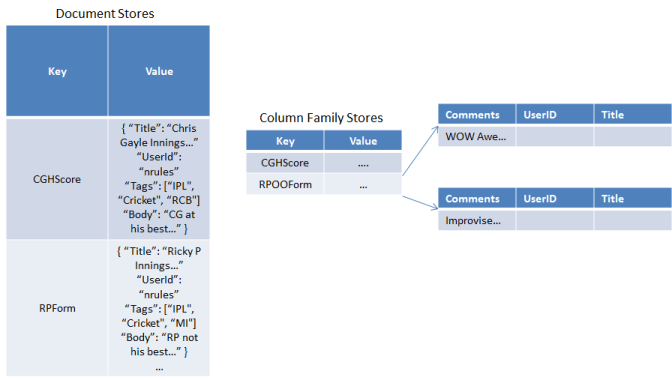
\includegraphics[width=0.8\textwidth]{columnnosql}
    \caption{Exemplo de estrutura de um NoSQL orientado a colunas.}
    \label{fig:columnnosql}
\end{figure}
	
\subsubsection{SGBD NoSQL orientado a documentos}
	Nessa categoria, os dados são armazenados em forma de documentos. Um documento dentro desse tipo de SGBD pode ser comparado a um registro dentro de um SGBD relacional, mas nos SGBD NoSQL existe uma flexibilidade maior pois é permitido uma estrutura \textit{Schema-less}. Normalmente, esses documentos seguem algum formato padrão como \textit{JSON} ou \textit{XML} por exemplo. Uma diferença com o formato dos bancos relacionais, é que um campo de um registro dentro de um SGBD relacional que não está preenchido, necessariamente ficará vazio, já num SGBD NoSQL orientado a documentos, cada documento pode ter dados similares ou não tão similares, ou seja, um campo sem informação não precisa aparecer como vazio para o usuário, demonstrando a flexibilidade que esses SGBD proporcionam \cite{nayak2013type}.
	
	Cada documento é endereçado por uma chave, da mesma forma que em SGBD NoSQL orientado a chave/valor. Esses SGBD são úteis em aplicações em que os dados não precisam ser armazenados em tabelas com campos uniformes, mas sim armazenados em documentos com características especiais. Normalmente, não é recomendado para dados com muitos relacionamentos ou normalização. Dois representantes dessa categoria são o MongoDB e o CouchDB \cite{nayak2013type}. A figura \ref{fig:columnnosql} mostra um exemplo da estrutura de um SGBD orientado a documentos em contraste com um SGBD orientado a colunas.
	
\subsubsection{SGBD NoSQL orientado a grafos}
	Os SGBD NoSQL orientado a grafos armazenam os dados em uma estrutura de grafo. As características e informações acerca da estrutura de um grafo são abordadas em maiores detalhes na seção \ref{graph_theory}. Resumidamente, um grafo é um conjunto de nós e arestas, em que os nós são os objetos e as arestas representam o relacionamente entre dois objetos (nós). Esses SGBD usam a técnica conhecida como  \textit{index free adjacency}, em que cada nó possui um ponteiro diretamente para nós adjacentes. Essa técnica permite que uma grande quantidade de nós seja percorrida de forma eficiente \cite{nayak2013type}. A figura abaixo exemplifica o formato de um grafo no SGBD NoSQL OrientDB.

\begin{figure}[h]
	\centering
    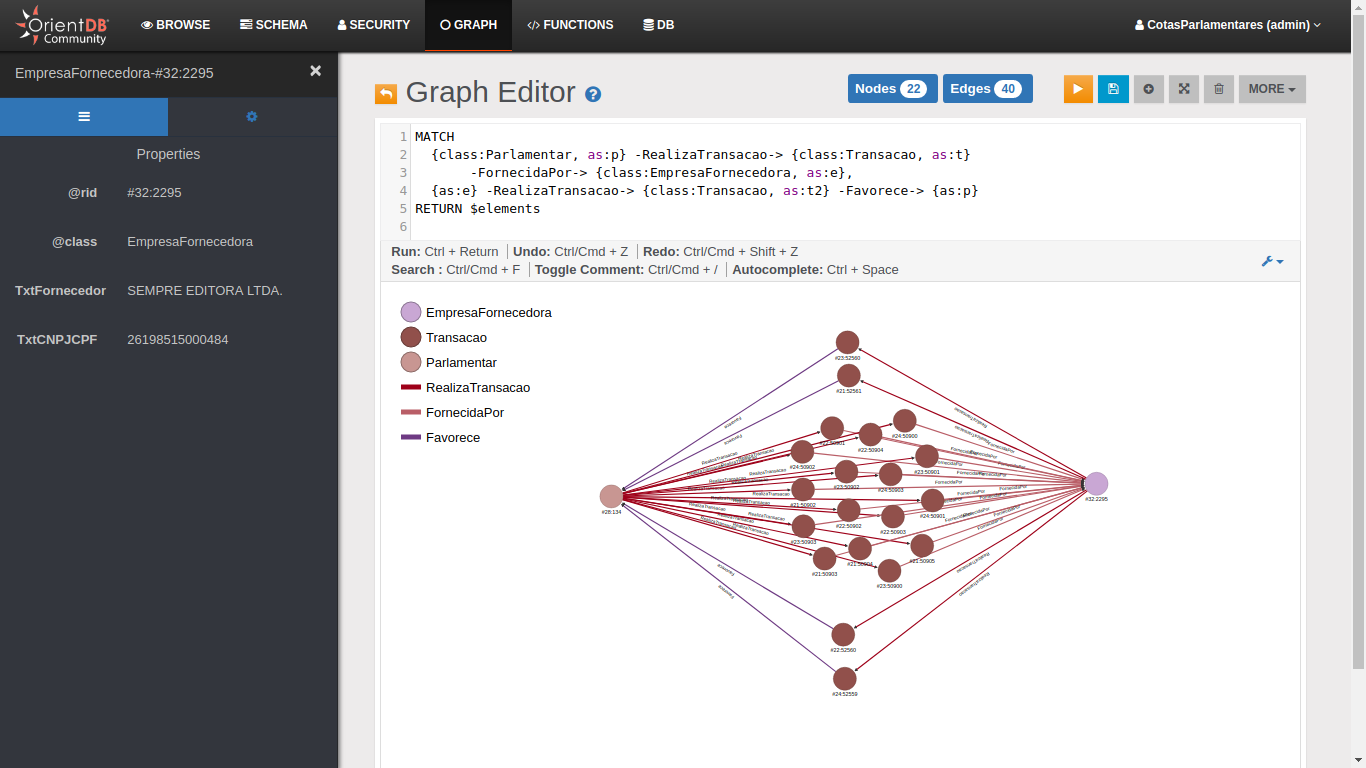
\includegraphics[width=0.8\textwidth]{orient_graph}
    \caption{Exemplo da estrutura de um grafo no SGBD OrientDB}
    \label{fig:graph_orientdb}
\end{figure}
	
	As consultas são feitas seguindo a ideia de percorrimento do grafo, o que torna esses SGBD mais eficientes que SGBD relacionais. O seu uso varia de aplicações para redes sociais, bioinformática, software de recomendação e etc \cite{nayak2013type}. O principal ponto de seu uso é em dados que são bastante relacionados entre si, pois a estrutura de um grafo expõe naturalmente os relacionamentos entre os objetos. O maior representando dessa categoria de SGBD é o Neo4j seguido pelo OrientDB e AllegroGraph.
	
\subsubsection{SGBD NoSQL orientado a objetos}
	Um SGBD orientado a objetos, armazena os dados e informações em objetos, similares aos objetos presentes no paradigma de orientação a objetos. Portanto, essa categoria de SGBD pode ser vista como uma combinação entre os princípios de programação orientada a objetos e banco de dados. Esses banco de dados oferecem todas as característica da programação orientada a objetos tais como: Encapsulamento de dados, polimorfismo e herança. É possível fazer um paralelo entre classe, objeto e atributos da classe com tabela, tupla e colunas em uma tupla dos banco de dados relacionais respectivamente \cite{nayak2013type}.
	
	Cada objeto nessa estrutura possui um identificador único que o representa. O acesso nessa estrutura é mais rápido pois cada objeto pode ser acessado através de ponteiros. O seu uso auxilia no processo de desenvolvimento de software, sendo útil também em aplicações envolvendo relacionamentos complexos entre objetos. Esse tipo de SGBD vem sendo usando em pesquisas científicas, telecomunicações e outras aplicações. Essa categoria tem a desvantagem de estar associada a um tipo específico de linguagem de programação e por possuir dificuldades de escalabilidade, uma vez que o tamanho da memória física é excedido \cite{nayak2013type}. Um grande representante dessa categoria é o db4o, o trabalho de Kulshrestha, Sudhanshu and Sachdeva e Shelly \cite{kulshrestha2014performance} faz uma comparação de performance entre SGBD relacionais e o db4o. A figura abaixo exemplifica como um objeto é dividído para ser armazenado em tabelas em uma estrutura relaciona, já na estrutura orientada a objetos, o objeto é armazenado sem essa divisão \cite{edlich2006definitive}.
	
\begin{figure}[h]
	\centering
    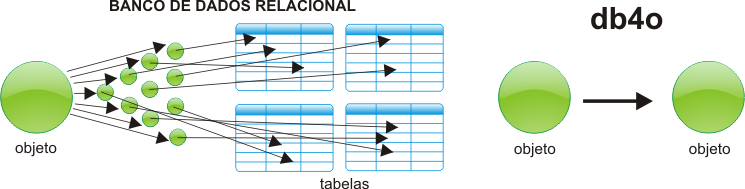
\includegraphics[width=0.8\textwidth]{Banco_Dados_Relacional_X_db4o_ver2}
    \caption{Contraste entre estrutura relaciona e orientada a objetos}
    \label{fig:db4o}
\end{figure} 

%%%%%%%%%%%%%%%%%%%%%%%%%%%%%%%%%%%%%%%%%%%%%%%%%%%%%%%%%%%%%%%%%%%%%%%%%%%%%%%%
%%%%%%%%%%%%%%%%%%%%%%%%%%%%%%%%%%%%%%%%%%%%%%%%%%%%%%%%%%%%%%%%%%%%%%%%%%%%%%%%
%%%%%%%%%%%%%%%%%%%%%%%%%%%%%%%%%%%%%%%%%%%%%%%%%%%%%%%%%%%%%%%%%%%%%%%%%%%%%%%%
\section{Comparação qualitativa entre OrientDB e Neo4j} \label{comparison_graph_nosql}

\subsection{Introdução}

	Hoje no mercado existem diversos SGBD orientado a grafos, tais são: OrientDB, Neo4j, AllegroGraph, FlockDB entre outros. Dentre esses, sem dúvida o mais popular é o SGBD NoSQL neo4j. Como foi mencionado no capítulo \ref{chap:1}, os SGBD orientado a grafos vem obtendo um grande número de novos usuários \cite{Dbmspopularity}, registrando a maior taxa de mudança de popularidade entre 2013 e 2017. Hoje o Neo4j se encontra na primeira posição segundo o seguinte ranking \cite{neo4jprimeiro}, e por esse motivo o seguinte capítulo realiza uma comparação entre o OrientDB e o Neo4j.
	
	Trabalhos como o de Jouili \cite{jouili2013empirical}, Kolomivcenko \cite{kolomivcenko2013experimental} e Kovacs \cite{kovacs2016cassandra}, realizam comparações entre os dois SGBD. Nessas comparações são levados em conta aspectos como performance, licensa comercial ou \textit{open source}, linguagem de consulta e etc. Além desses trabalhos, artigos como o de Barmpis \cite{barmpis2014evaluation} e Labute \cite{labute2014review} reforçam o fato do crescimento tanto no uso comercial quanto em pesquisas acadêmicas em banco de dados orientado a grafos.
	
\subsection{Comparação qualitativa}

	O trabalho feito por Angles \cite{angles2012comparison} em 2012 compara alguns SGBD orientado a grafos. Foi identificado três características comuns entre todos os modelos que são: O esquema e as instâncias são modelados como grafos, operações orientada a grafos e um conjunto de regras de integridade. Dessa forma, a tabela \ref{table:1} representa uma comparação entre os modelos de dados do OrientDB e Neo4j:
	
\begin{table}[h!]
\centering
\begin{tabular}{|l|l|l|l|l|}
\hline
SGBD                        & OrientDB                                                                        & Neo4j \\ \hline
Modelo de banco de dados    & \textit{multi-model DBMS}                                                       & \textit{Graph DBMS}  \\ \hline
Modelos de esquema          & \makecell{\textit{Schema-full},\\ \textit{Schema-less},\\ \textit{Schema-hybrid}} & \textit{schema-free} e \textit{schema-optional} \\ \hline
Tipos de dados customizados & Sim                                                                             & Não \\ \hline
Modelo Reativo              & Sim                                                                             & Não \\ \hline
\end{tabular}
\caption{Comparação qualitativa entre modelo de dados do OrientDB e Neo4j}
\label{table:1}
\end{table}

	Portanto, podemos observar que o OrientDB é um SGBD multi modelo, pois suporta operações com documentos, chave/valor e grafos. Já o Neo4j trabalha somente com o modelo de grafos. Além disso, o OrientDB possui suporte para diferentes modelos de esquema podendo usar um esquema completo, nenhum esquema ou um esquema híbrido para modelar os dados. O Neo4j se utiliza nenhum esquema na modelagem ou um esquema opcional, baseado no conceito de labels. Nesse esquema opcional, os labels são usados na especificação de índices, e para definir restrições no grafo, juntos ambos formam o esquema do grafo no Neo4j \cite{neo4jschemaoptional}. O OrientDB permite que o usuário crie tipo de dados customizados no esquema, basta que a classe da propriedade já exista no banco de dados \cite{orientdbcreateproperty}, enquanto no Neo4j isso não é possível. Finalmente, uma característica interessante que o OrientDB fornece é a de modelo reativo. Essa propriedade é chamada de \textit{live query} \cite{orientdblivequery}, e é utilizada para construir aplicações em tempo real. Em uma abordagem tradicional, é inviável que o cliente da aplicação fique o tempo inteiro realizando consultas para obter novas atualizações, pois isso gera um grande desperdício de recursos. A imagem \ref{fig:orientdbReativo} resume a situação:
	
\begin{figure}[H]
	\centering
    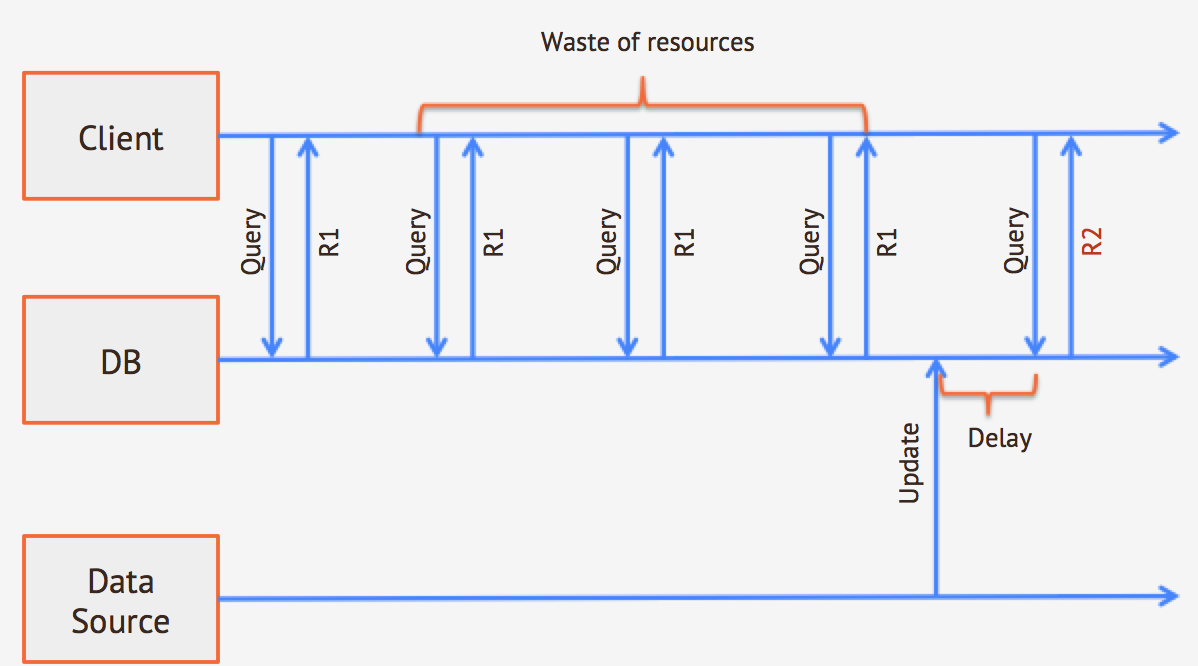
\includegraphics[width=0.8\textwidth]{queryPolling}
    \caption{Exemplo de tentativa de aplicação reativa}
    \label{fig:orientdbReativo}
\end{figure}

\begin{figure}[H]
	\centering
    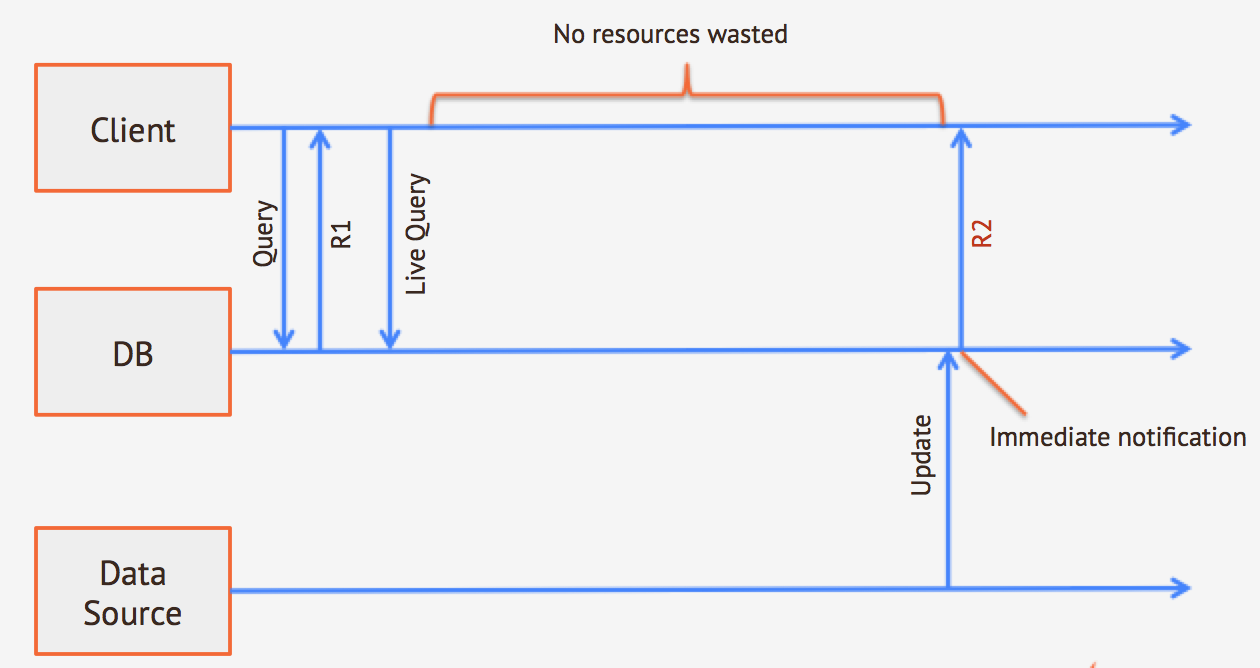
\includegraphics[width=0.8\textwidth]{liveQuery}
    \caption{Exemplo do uso de \textit{live queries}}
    \label{fig:orientDBLiveQuery}
\end{figure}

	Com o uso das \textit{live queries}, esse tipo de problema é resolvido e não há mais desperdício de recursos, como mostra a figura \ref{fig:orientDBLiveQuery}.

	Apesar de várias diferenças, os dois SGBD possuem características em comum. A tabela \ref{table:2} demonstra comparações de características gerais, entre o OrientDB e o Neo4j:
	
\begin{table}[h!]
\centering
\begin{tabular}{|l|l|l|l|l|}
\hline
SGBD                       & OrientDB                                    & Neo4j \\ \hline
Transações ACID            & Sim                                         & Sim \\ \hline
Suporte a dados espaciais  & Sim                                         & Sim \\ \hline
Licensa de uso             & Apache versão 2                             & GPL versão 3 \\ \hline
Linguagem implementada     & Java, Scala                                 & Java \\ \hline
Linguagem de consulta      & \makecell{Linguagem derivada do SQL,\\ sem uso de joins} & Cypher \\ \hline
Métodos de particionamento & Sharding                                    & Não \\ \hline
Metodos de replicação      & Multi-master replication                    & \makecell{Causal Clustering \\ using Raft protocol} \\ \hline
Suporte a MapReduce        & Sim                                         & Não \\ \hline
Concorrência               & Sim                                         & Sim \\ \hline
\end{tabular}
\caption{Comparação qualitativa de características gerais entre OrientDB e Neo4j}
\label{table:2}
\end{table}

	A partir da tabela \ref{table:2}, é possível observar algumas características em comum entre os SGBD, por exemplo, ambos trabalham com o modelo de transações ACID, que foi discutido em detalhes na seção \ref{manage_transaction}. Além disso, os dois suportam o uso de dados e consultas espaciais para trabalhar com dados geográficos, cada um possui uma versão open source, mesmo que sob licensas diferentes. É importante pontuar também que ambos possuem suporte a acessos concorrentes e foram desenvolvidos utilizando a linguagem de programação Java.
	
	Uma diferença importante entre os dois SGBD é em relaçao a linguagem de consulta utilizada. O OrientDB possui uma linguagem de consulta derivada da linguagem SQL, isso é bastante vantajoso para aqueles que vem do universo de SGBD relacional, enquanto o Neo4j utiliza uma linguagem de consulta própria conhecida como cypher. O código abaixo exemplifica uma consulta no OrientDB e sua semelhanças com consultas de bancos de dados relacionais:
	
\begin{lstlisting}[label={lst:labelSQL}, caption={Exemplo de consulta no SGBD OrientDB},captionpos=b, language=sql]
SELECT FROM Person WHERE name LIKE 'Luk%'
\end{lstlisting}

	A consulta acima retorna todas as instâncias da classe Person onde o atributo name começa com a \textit{string} 'Luk'. Finalmente, no que diz respeito a arquitetura distribuída, o OrientDB possui suporte em sua versão open source, enquanto o Neo4j possui suporte somente na licensa comercial. O OrientDB utiliza o método de \textit{sharding} para separar os dados em clusters diferentes, enquanto o Neo4j não possui suporte para esse tipo de funcionalidade. Em relação aos métodos de replicação o OrientDB trabalha com o modelo multi-master, discutido em detalhes na seção \ref{orient_distributed}, e o Neo4j utiliza o método \textit{Causal Clustering using Raft protocol} \cite{neo4jcausal}. Por possuir suporte a funcionalidade de \textit{sharding}, o OrientDB também suporta operações de MapReduce sem o uso de tecnologias como o Hadoop ou Spark. Essa funcionalidade é totalmente transparente para o desenvolvedor, de forma que quando uma consulta envolve múltiplos clusters, o SGBD executa a query sobre cada nó (Operação de Map) e em seguida realiza o \textit{merge} dos resultados (Operação de reduce) \cite{orientMapReduce}.
	
\subsection{Conclusão}

	Portanto, em vista dos fatos mencionados, o OrientDB possui uma quantidade de funcionalidades maior que o Neo4j, principalmente em sua versão comunitária, ou open-source. Funcionalidades importantes como o uso de uma arquitetura distribuída, estão presentes somente na versão comercial do Neo4j, o que fez com que o OrientDB fosse escolhido para uso no estudo de caso. O fato de possuir uma linguagem próxima ao SQL, também pesou na escolha, pois proporciona uma produtividade maior para aqueles acostumados com a linguagem de consulta SQL.
	
	Outra característica pouco pontuada, mas bastante importante, é a presença de uma comunidade por trás da tecnologia para auxiliar os desenvolvedores. A comunidade por trás do OrientDB é grande e bastante presente em sites como o \textit{StackOverflow} \cite{orientStack} e \textit{Linkedin}, inclusive com presença do próprio \textit{CEO} da empresa em ambos os \textit{sites}. Contudo, é inquestionável que o Neo4j é mais popular entre desenvolvedores e possui uma comunidade maior que a do OrientDB, o que sem dúvida é uma vantagem competitiva.
	
	Uma conclusão em relação a qual tecnologia é melhor, seria que no geral ambas são igualmente boas com pontos positivos e negativos para cada lado. O fato do Neo4j possuir uma comunidade maior é bastante importante, mas o fato de poder utilizar um SGBD com arquitetura distribuída gratuitamente também tem sua importância. A escolha entre um ou outro deve ser ponderada de projeto a projeto, e para esse trabalho foi escolhido o OrientDB pelo motivos pontuados no início dessa seção.

%%%%%%%%%%%%%%%%%%%%%%%%%%%%%%%%%%%%%%%%%%%%%%%%%%%%%%%%%%%%%%%%%%%%%%%%%%%%%%%%
%%%%%%%%%%%%%%%%%%%%%%%%%%%%%%%%%%%%%%%%%%%%%%%%%%%%%%%%%%%%%%%%%%%%%%%%%%%%%%%%
%%%%%%%%%%%%%%%%%%%%%%%%%%%%%%%%%%%%%%%%%%%%%%%%%%%%%%%%%%%%%%%%%%%%%%%%%%%%%%%%
\section{OrientDB} \label{OrientDBMain}

	Essa seção tem por objetivo especificar as características do SGBD OrientDB, e realizar uma comparação com outros SGBD orientado a grafos como o Neo4j.
	
\subsection{Introdução}
	
	O OrientDB, é um SGBD de código aberto sob a licensa Apache. Ele é o primeiro SGBD NoSQL multi modelo, com suporte a uma arquitetura distribuída e orientado a grafos. Sendo assim o OrientDB suporta operações com documentos, chave/valor e grafos. Essa característica garante uma enorme flexibilidade para manipular os dados dentro do OrientDB, sendo possível armazenar os dados tanto como grafos ou como documentos no mesmo banco de dados \cite{OrientDB}. A figura a seguir resume as possibilidades de registros no OrientDB:
	
\begin{figure}[h]
	\centering
    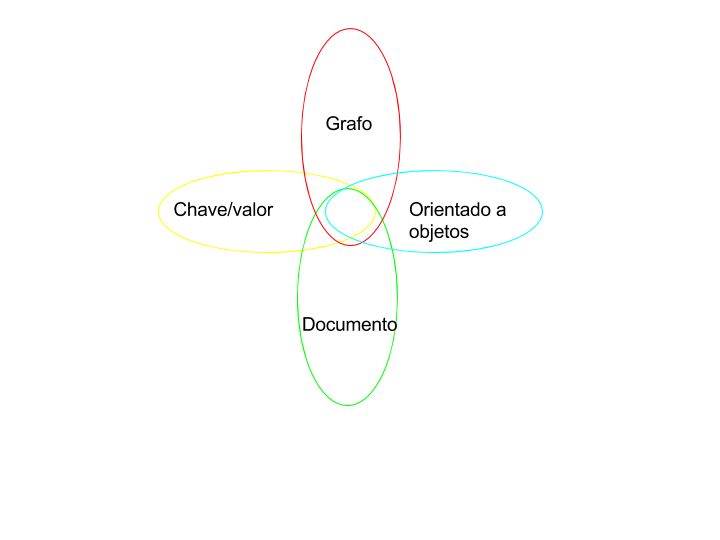
\includegraphics[width=0.8\textwidth]{orientdbmodel}
    \caption{Possibilidade de registros no OrientDB}
    \label{fig:orientdbpossibilities}
\end{figure}
	
	O OrientDB é implementado utilizando a linguagem java, tendo sua primeira versão disponível no ano de 2010. Ele possui alta flexibilidade para definir o esquema do banco de dados, podendo ser \textit{Schema-free}, \textit{Schema-hybrid} ou \textit{Schema-full}. A sua linguagem de consulta é derivada do SQL o que é bastante vantajoso para aqueles que possuem experiência com bancos de dados relacionais, e além disso ele utiliza o modelo de transações ACID que como foi mencionado na seção \ref{manage_transaction} é algo mais comum no grupo dos SGBD relacionais, isso demonstra que o OrientDB presa pela integridade dos dados ao mesmo tempo que também fornece um suporte a particionamento dos dados \cite{OrientDB} \cite{vschart}.
	
	Todas essas características fazem com que o OrientDB seja um SGBD bastante flexível e confiável para se utilizar em diversas aplicações. As operações utilizando grafos em específico, vem ganhando bastante visibilidade pois funciona muito bem em certos domínios de aplicação. Como foi mencionado no capítulo \ref{chap:1} e nesse artigo feito por Matthias Gelbmann \cite{Graphpopularity} a popularidade dos SGBD orientados a grafos vem crescendo bastante nos últimos anos, e essas características ajudam a explicar o porque de banco de dados como o OrientDB e Neo4j estarem crescendo tanto em popularidade.
	
\subsection{Performance} \label{orient_performance}
	O OrientDB possui uma ótima performance em operações utilizando grafos. Um aspecto técnico que ajuda nessa qualidade é que o OrientDB trabalha cada registro como um objeto e o \textit{link} entre esses objetos não é feito por referência, e sim por \textit{link} direto. Ou seja, é salvo um ponteiro que aponta diretamente para o objeto referenciado. Isso faz com que a velocidade para recuperar informações seja muito mais rápido em comparação com os joins utilizados nos SGBD relacionais. Portanto, não existem operações de joins dentro do OrientDB para obter as relações entre os registros, sendo que ele consegue salvar certa de 120 mil registro por segundo.
	
	O OrientDB utiliza mecanismos de indexação baseados em árvores-B e hash extendido, esses mecanismos garantem uma complexidade constante para obter relacionamentos entre um registro para muitos registros. Um estudo feito pelo instituto de tecnologia de tokio e pela IBM, mostra que o OrientDB chega a ser 10 vezes mais rápido que o seu maior concorrente que é o Neo4j \cite{dayarathna2012xgdbench}.
	
	O trabalho feito po Toyotaro Suzumura e Miyuru Dayarathna \cite{dayarathna2012xgdbench}, aponta como a estrutura de grafos vem crescendo em sistemas na nuvem, devido ao crescimento de aplicações que produzem dados em formato de grafos, como aplicações de web semântica, sistemas de informação geográfico (GIS), aplicação de bioinformática \cite{dudley2010translational} e química informática \cite{ekins2010chemical}. Sendo que históricamente, dados com estrutura de grafos eram modelados com relacionamentos e armazenados em bases relacionais. Toda a lógica de percorrimento de grafos ficava para outras camadas da aplicação. Entretanto, percebe-se que o armazenamento desse tipo de dado e a análise feita em cima dessa estrurura feita nos SGBD são mais eficientes, uma vez que fornecem uma performance otimizada e produtividade na especificação de consultas \cite{dayarathna2012xgdbench}.
	
	Um dos objetivos desse artigo \cite{dayarathna2012xgdbench} é realizar um benchmark e estudar a performance de quatro grandes SGBD orientado a grafos em ambiente de nuvem. Os SGBD são AllegroGraph \cite{allegro}, Fuseki \cite{fuseki}, Neo4j \cite{neo4j-site} e o OrientDB \cite{orientdb-site}. Eles utilizaram o XGDBench que é uma extensão do conhecido Yahoo! Cloud Serving Benchmark (YCSB). O YCSB é um framework de benchmark para sistemas na nuvem. Foram criados cinco \textit{Workloads} para realizar os testes:

\begin{itemize}
	\item  \textit{Update heavy}: 50/50 entre leitura e atualizações
	\item  \textit{Read mostly}: 95/5 entre leitura e atualizações
	\item  \textit{Read only}: 100 por cento de leituras
	\item  \textit{Read latest}: esse \textit{Workload} insere novos vértices ao grafo
	\item  \textit{Short Ranges}: esse \textit{Workload} lê todos os vizinhos e seus atributos de um dado vértice A.
\end{itemize}

	Em todos os workloads, levando em conta a arquitetura e o hardware utilizado no ambiente de nuvem, o OrientDB teve um desempenho melhor que os demais SGBD \cite{dayarathna2012xgdbench}.
	
	
\subsection{Arquitetura Distribuída} \label{orient_distributed}
	Em relação ao suporte a uma arquitetura distribuída, o OrientDB trabalha com um método de particionamento conhecido como \textit{sharding}, e um método de replicação conhecido como \textit{Multi-master replication}. Esse modelo de replicação, permite que qualquer membro do cluster possa ler e escrever no banco de dados. Essa arquitetura permite que exista uma escalabilidade horizontal sem gargalos, como ocorre em algumas outras soluções de SGBD NoSQL \cite{kauremerging}.
	
	No ano de 2012 o OrientDB trabalhava com uma arquitetura diferente, conhecida como \textit{Master-slave replication}. A figura a seguir exemplifica o formato dessa arquitetura.
	
\begin{figure}[h]
	\centering
    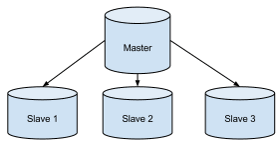
\includegraphics[width=0.5\textwidth]{master-slave}
    \caption{Exemplo de uma arquitetura \textit{Master-slave}}
    \label{fig:master-slave}
\end{figure}

	Esse tipo de arquitetura é eficiente para escalar as operações de leituras, mas também é importante conseguir escalar as operações de escrita no banco de dados. Como é possível ver na imagem acima, um nó (\textit{Master}) é responsável por receber as requisições de leitura e distribuir essa operações entre os demais nós \textit{Slaves}. Porém, ao projetar dessa forma o nó \textit{Master} se torna um gargalo para a aplicação, de forma que, ao receber muitas requisições o nó passa a ficar sobrecarregado.
	
	Uma vantagem dessa arquitetura, é sua facilidade de implementação, pois basta realizar o roteamento das requisições entre os nós \textit{Slaves}. Como desvantagens temos o fato do nó \textit{Master} ser o gargalo nas operações de escrita, e a característica de que não adianta aumentar a quantidade de servidores para aumentar a vazão, pois a vazão é inevitavelmente limitada pelo nó \textit{Master}.
	
\begin{figure}[h]
	\centering
    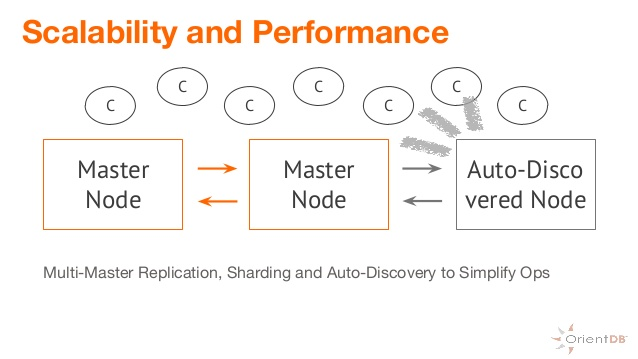
\includegraphics[width=0.5\textwidth]{orientdb-the-2nd-generation-of-multimodel-nosql-44-638}
    \caption{Exemplo de uma arquitetura \textit{Multi-master}}
    \label{fig:multi-master}
\end{figure}
	
	Nesse cenário, o SGBD evoluiu para a arquitetura \textit{Multi-master} representada pela figura acima. Nesse formato, todos os nós de um cluster aceitam operações de escrita. Além desse formato, o SGBD passou a adotar o método de particionamento conhecido como \textit{sharding}, em que os dados são divididos em múltiplas partições. Como é mencionado na seção \ref{orient_object}, o conceito de classes é bastante útil na arquitetura distribuída, uma vez que por padrão para cada classe criada o SGBD cria um cluster para que suas instâncias sejam armazenadas. Combinando essas técnicas, o OrientDB proporciona uma escalabilidade tanto em leituras quanto em escritas. Uma vantagem desse modelo é que se um nó \textit{Master} falhar, os demais podem continuar a operar normalmente.

\subsection{Orientação a Objetos} \label{orient_object}

	Uma das características mais interessantes do OrientDB é o suporte que ele da para que o usuário organize os seus dados seguindo padrões de orientação a objetos. Como foi mencionado na seção \ref{orient_performance}, o OrientDB considera cada registro como um objeto, dessa forma é possível criar classes que representam a estrutura dos dados. Por exemplo, no capítulo 3 eu explico um pouco mais sobre como fiz a modelagem dos dados seguindo o modelo MDG-NoSQL proposto por Gustavo C. Galvão Van Erven\cite{mdgnosql}. Nessa modelagem eu identifiquei as seguintes classes Transação, Empresa fornecedora, Parlamentar e Pessoa. O OrientDB permite que eu crie essas classes e ao inserir um vértice eu especifique que esse vértice é de uma classe específica, isso facilita bastante na hora de escrever as consultas pois basta utilizar o nome da classe que todos os vértices pertencentes a essa classe serão obtidos. O conceito de classe também se aplica as arestas, e tudo isso facilita na organização dos dados e na escrita de consultas ao banco de dados.
	
	Um registro é a menor unidade que é possível salvar e obter no banco de dados do OrientDB, ele pode ser obtido de quatro formas:
	
	\begin{itemize}
		\item Documento
		\item \textit{RecordBytes} (BLOB)
		\item Vértice
		\item Aresta
	\end{itemize}
	
	Dessa forma, uma classe para esse tipo de registro, é o conceito mais próximo de tabela existente no OrientDB. O conceito de herança, muito utilizado no paradigma orientado a objetos, também possui suporte no OrientDB, sendo que classes podem herdar atributos e propriedades de uma classe pai. Por exemplo, a classe pessoa mencionada acima, pode ser a classe pai da classe parlamentar, assim um parlamentar herda atributos de pessoa. Além disso, ao realizar uma consulta utilizando a classe pessoa, automaticamente todos os parlamentares também serão utilizados. Outra funcionalidade atrelada a esse assunto, é o suporte a classes abstratas utilizadas para definir outras classes. Uma classe abstrata não possui instâncias no banco de dados, bastante similar com os conceitos em orientação a objetos. 
	
	A figura a seguir exemplifica a herança presente no OrientDB, no caso é possível criar três classes para armazenar as instâncias dos vértices, que são: \textit{Employee}, \textit{Regular employee} e \textit{Contract employee}. As duas últimas classes herdam os atributos id e name da classe pai, sendo que ao realizar uma busca por todos as instâncias de \textit{Employee}, tanto \textit{Regular employee} quanto \textit{Contract employee} serão retornados.
	
\begin{figure}[h]
	\centering
    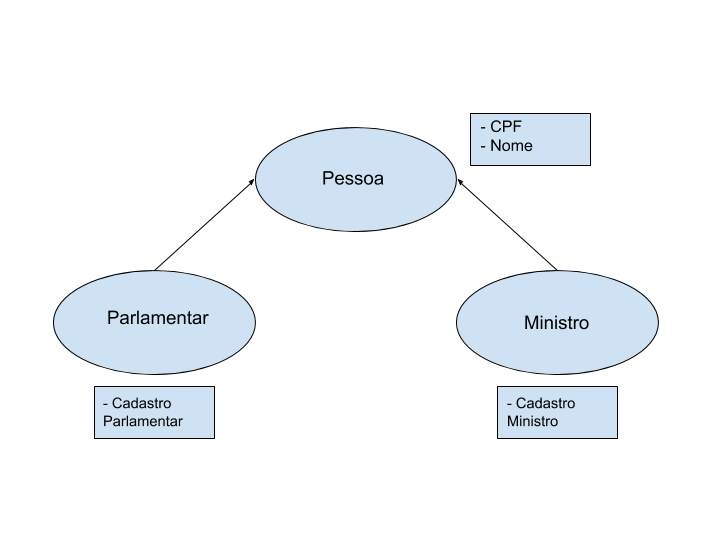
\includegraphics[width=0.5\textwidth]{teleporter-inheritance-orientdb-schema}
    \caption{Exemplo de herança no \textit{schema} do OrientDB }
    \label{fig:inheritance-orient}
\end{figure}
	
	Para finalizar é importante mencionar que as classes tem um papel importante ao se utilizar a arquitetura distribuída no OrientDB, pois para cada classe criada, o SGBD cria um cluster automaticamente para armazenar instâncias dessas classes. Essa funcionalidade auxilía bastante na organização do particionamento dos dados em um ambiente distribuído. Todos os registros de uma classe são armazenados juntos no mesmo cliuster que tem o mesmo nome da classe. No OrientDB é possível criar até trinta e dois mil setecentos e setenta e sete clusters. Compreender bem os conceitos de classes nesse SGBD, permite que o usuário tenha vantagem ao fazer o \textit{design} do banco de dados. Vale lembrar que uma classe pode ser mapeada para n clusters como mostra a figura a seguir:
\begin{figure}[h]
	\centering
    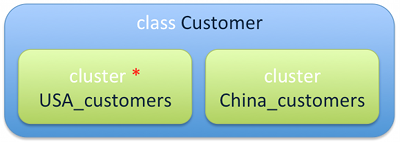
\includegraphics[width=0.5\textwidth]{class-clusters}
    \caption{Classe Customer mapeada para dois clusters diferentes}
    \label{fig:class-cluster}
\end{figure}

%%%%%%%%%%%%%%%%%%%%%%%%%%%%%%%%%%%%%%%%%%%%%%%%%%%%%%%%%%%%%%%%%%%%%%%%%%%%%%%%
%%%%%%%%%%%%%%%%%%%%%%%%%%%%%%%%%%%%%%%%%%%%%%%%%%%%%%%%%%%%%%%%%%%%%%%%%%%%%%%%
%%%%%%%%%%%%%%%%%%%%%%%%%%%%%%%%%%%%%%%%%%%%%%%%%%%%%%%%%%%%%%%%%%%%%%%%%%%%%%%%
\section{\textit{REST}}

\subsection{Introdução} \label{rest_intro}

	O termo \textit{REST} significa \textit{Representational State Transfer}, em português Transferência de Estado Representacional, e foi introduzido por Roy Fielding em sua tese de doutorado \cite{fielding2000architectural}. Como Roy Fielding afirma em sua tese, a complexidade dos sistemas de \textit{software} modernos fazem necessário uma ênfase maior  em sistemas componentizados, em que a implementação é dividida em componentes independentes que se comunicam para realizar uma tarefa desejada \cite{fielding2000architectural}.
	
	Ainda em sua tese, Roy Fielding explora o encontro entre duas discplinas da área de ciência da computação: \textit{software} e \textit{networking}. Ele afirma que as pesquisas de softwares se preocupavam em categorizar o \textit{desing} de \textit{software}, e desenvolver novas metodologias de \textit{desing}, em vez de avaliar o impacto das decisões de \textit{design} no comportamento de um sistema. Enquanto as pesquisas de \textit{networking}, foca nos detalhes da comunicação genérica entre sistemas e em melhorar a performance de uma técnica de comunicação específica, muitas vezes ignorando o fato de que mudar o estilo de interação de uma aplicação pode gerar mais impacto na performance, do que quais protocolos de comunicação são usados nessa interação \cite{fielding2000architectural}.
	
	Portanto, nesse contexto, o trabalho de Roy Fielding tinha como objetivo entender e avaliar o \textit{design} arquitetural de uma aplicação de software baseada na rede através do uso de restrições arquiteturais, dessa forma obtendo as propriedades sociais, performáticas e funcionais que se espera de uma arquitetura \cite{fielding2000architectural}. Dessa forma, o \textit{REST} é um estilo de arquitetura para sistemas hipermídia distribuídos. O \textit{REST} provê um conjunto de restrições arquiteturais que ao serem aplicadas, enfatizam a escalabilidade das interações entre componentes, generalidade de interfaces, \textit{deploy} independente dos componentes e componentes intermediários para reduzir a latência nas interações, reforçar a segurança e encapsular sistemas legados \cite{fielding2000architectural}.
	
\subsection{Princípios do estilo arquitetural \textit{REST}}

	A característica principal que diferencia o \textit{REST} de outros estilos baseados em rede, é a ênfase em uma interface uniforme entre os componentes. Dessa forma, a arquitetura geral do sistema é simplificada e a visibilidade das interações e melhorada. Entretanto, um problema nesse princípio é que a eficiência se torna pior. Isso ocorre, pois, a informação é transferida de forma padronizada, em vez de um formato específico a necessidade das aplicações \cite{fielding2000architectural}.
	
	Como foi dito na seção \ref{rest_intro}, o estilo arquitetural \textit{REST} impõe uma série de restrições ao sistema. Portanto, o \textit{REST} possui alguns princípios que os sistemas devem adotar para serem considerados \textit{RESTful}, que são: 

\begin{itemize}
	\item Todos os componentes do sistema se comunicam através de interfaces com métodos bem definidos e código dinâmico. A comunicação entre os componentes utiliza o protocolo \textit{HTTP}.
	\item Cada componente é unicamente identificado por um link hipermídia (URL)
	\item Uma arquitetura cliente/servidor \textit{stateless} é seguida.
	\item A arquitetura possui camadas, e os dados podem ser cacheados em qualquer camada.
\end{itemize}

	Atualmente, vários serviços na web fornecem interfaces \textit{REST}, para que interessados possam consumir os dados, tais como a Amazon, eBay, Yahoo. A câmara dos deputados também utiliza o estilo arquitetural \textit{REST} para fornecer algumas informações. Além disso, o framework \textit{ruby on rails}, que foi utilizado para desenvolver o sistema do estudo de caso, suporta aplicações \textit{REST} utilizando o padrão MVC.
	
	Um ponto interessante a ser colocado, é que nem todas essas aplicações mencionadas são puramente \textit{REST}, pois não respeitam todas as restrições destacadas por Roy Fielding em sua tese \cite{fielding2000architectural}. Esses serviços, seguem os princípios mais importantes, principalmente a interface uniforme. Tais aplicações são conhecidas como "acidentalmente \textit{RESTful}" \cite{acident-rest}.

	A figura abaixo exemplifica o estilo arquitetural \textit{REST}:

\begin{figure}[h]
	\centering
    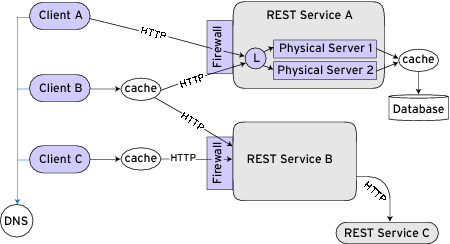
\includegraphics[width=0.5\textwidth]{rest}
    \caption{Estilo arquitetural \textit{REST}}
    \label{fig:rest-style}
\end{figure}


\subsection{Interface \textit{REST} no OrientDB} \label{rest_orient_db}
	O SGBD orientado a grafos utilizado no estudo de caso foi o OrientDB, descrito em mais detalhes na seção \ref{OrientDBMain}. O OrientDB fornece uma interface \textit{REST} de forma que as aplicações se comuniquem com o SGBD de forma eficiente e escalável. Essa interface utiliza os métodos do protocolo \textit{HTTP} para realizar operações nos dados, como descrito abaixo:
	
\begin{itemize}
	\item Método GET: Utilizado para recuperar dados do banco de dados. É uma operação idempotente, isso significa que nenhuma mudança no banco de dados é feita.
	\item Método POST: Utilizado para persistir dados no banco de dados.
	\item Método PUT: Utilizado para atualizar dados já persistidos no banco de dados.
	\item Método DELETE: Utilizado para deletar dados já persistidos no banco de dados.
\end{itemize}

	Dessa forma, uma aplicação que deseja se conectar ao SGBD utilizando a interface \textit{REST}, realizaria o seguinte comando: 
	
\begin{lstlisting}[label={lst:label_rest_get}, caption={Exemplo de conexão com o OrientDB utilizando o protocolo HTTP.},captionpos=b]
GET http://{{server}}:{{port}}/connect/{{database}}
\end{lstlisting}

	Esse método se conecta com um servidor remoto usando o formato de autenticação básica. Basta fornecer o endereço e porta do servidor e o nome do banco de dados. Se tudo ocorrer corretamente uma resposta 204 OK é retornada.
	
	Se a aplicação deseja, por exemplo, obter todos os parlamentares persistidos no banco de dados, realizaria o seguinte comando:
	
\begin{lstlisting}[label={lst:label_rest_get_parlamentar}, caption={Exemplo de consulta no OrientDB utilizando o protocolo HTTP.},captionpos=b]
GET http://{{server}}:{{port}}/query/{{database}}/{{language}}/SELECT 
from Parlamentar
\end{lstlisting}

	Nesse caso, ao fornecer o endereço e porta do servidor, o nome do banco de dados e especificar a linguagem como sendo "sql", o SGBD retorna no formato JSON todos os parlamentares disponíveis no banco de dados.
%%%%%%%%%%%%%%%%%%%%%%%%%%%%%%%%%%%%%%%%%%%%%%%%%%%%%%%%%%%%%%%%%%%%%%%%%%%%%%%%
%%%%%%%%%%%%%%%%%%%%%%%%%%%%%%%%%%%%%%%%%%%%%%%%%%%%%%%%%%%%%%%%%%%%%%%%%%%%%%%%
%%%%%%%%%%%%%%%%%%%%%%%%%%%%%%%%%%%%%%%%%%%%%%%%%%%%%%%%%%%%%%%%%%%%%%%%%%%%%%%%